\documentclass{SBCbookchapter}
\usepackage[utf8]{inputenc}
\usepackage[T1]{fontenc}
\usepackage[brazil,english]{babel}
\usepackage{graphicx}
\title{Typhoon Prediction: A Supervised Machine Learning Approach}
\begin{document}
\maketitle

%\addcontentsline{toc}{chapter}{Statistics}

%\emph{Find a statistical method which uses only Japan Meteorological Agency (JMA) best track typhoon data during or before year $n$ to hind-cast the entire best track of all typhoons in years $n+1$.   Given only the latter typhoons' initial three best track points (i.e. at $t=0,6,$ and $12$ hours), the maximum position error at each hind-casted track point must be less than 500 km. The method must work for the three most recent years of published best track data.}

\vspace{.3in}
\begin{minipage}[r]{4.25in}{\small
  The enormous devastation caused by super typhoon Haiyan (2013) motivates us to consider whether data from past typhoons hold a key to predicting the grade (``category'') of an emerging tropical storm from early best track data (lat, lon, windspeed and pressure in the first 18 hours). In particular, we describe a machine learning (ML) approach to classification of typhoon grade as well as ML regression models of maximum wind speed. We train and validate our model and make 'hindcasts' using Japan Meteorological Agency (JMA) best-track data.}
\end{minipage}

\newpage

\section{Introduction}

  In November 2013, Typhoon Haiyan struck the Philippines with sustained wind speeds of nearly 200
miles per hour, claiming over 6,000 lives, displacing 4 million people, damaging over a million houses,
and resulting in a request for over 750 million dollars
in humanitarian aid. Devastation caused by
``super typhoons" like Haiyan makes the on-going
development of early warning systems an absolute
necessity to provide vulnerable communities sufficient preparation time to
mitigate damage to both life and property. This motivates us to apply Machine Learning algorithms to predict the typhoon grade (category model), and maximum wind speed (regression model).

\section{Overview of Supervised Machine Learning}

Supervised Machine learning (ML) refers to a set of algorithms which utilize a training data set to develop a model which takes one or more input variables called \emph{predictors} and outputs the value of a variable called a \emph{response}. We will use Japan Meteorological Agency (JMA) data for 2009-2014 as training data:

\begin{itemize}
	\item Predictor Variables: Lat, Lon, WS and Pressure at times $t=0,6,12,18$ hours.
	\item Response Variables: Typhoon grade (3,4, or 5) and maximum sustained wind speed.
\end{itemize}

 {\flushleft In the} next section we describe a number of different ML algorithms such as decision tree, k-nearest neighbor, ensemble. In this chapter, we do not consider \emph{unsupervised} ML algorithms where the response variables are not known in advance, and hence not specified in the training data set.



 When the response is a discrete set, such as is the case for typhoon grade, we use a \emph{categorical} ML algorithm. When the response is continuous, such as maximum wind speed, we use a \emph{regression} algorithm.  In both cases, the accuracy of the prediction is our primary performance measure.  
 
 In the case of categorical models, one way to report accuracy is via a \emph{confusion matrix}. Figure \ref{FineTreeCategorical} gives an example of the latter, for a model which on the training data set accurately classifies 13 grade, 13 grade 4, and 47 grade 5 typhoons. In addition, specific information about the classification errors is given.  For example, 8 typhoons predicted as grade 5 were actually grade 4, and 9 typhoons predicted as grade 4 were actually grade 5. 
 
  \begin{figure}[!htpb]
  	\centering
  	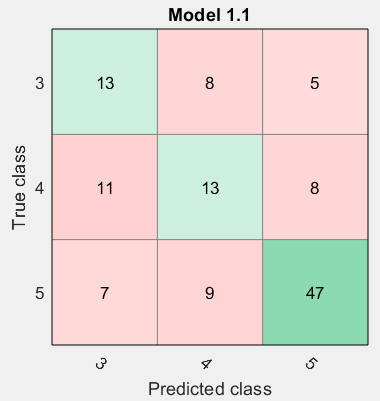
\includegraphics[width=3in,height=1.75in]{TyphoonCM1.png}
  	\caption{Confusion matrix for a typhoon grade Fine Tree categorical ML model.}
  	\label{FineTreeCategorical}
  \end{figure}
  
  
For a regression model, a scatter plot which compares the actual to the predicted values, with the difference between them called residuals is a standard visual representation of the error. The root mean squared error (RMSE) is calculated as the square root of the mean squared residuals. Figure \ref{FineTreeRegression} shows such a scatterplot, with in particular shows fairly good wind speed prediction of Grade 5 violent typhoon (maximum wind speeds of at least 105 knots/hr) as well as grade 3 tropical storms, but has greater difficulty in achieving accurate wind speed prediction for the typhoons in the mid-range (category 4).

\begin{figure}[!htpb]
	\centering
	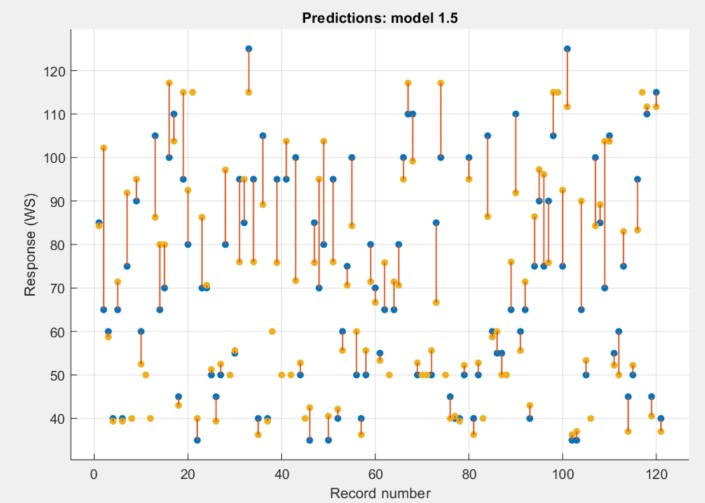
\includegraphics[width=3in,height=1.75in]{TyphoonCM2.png}
	\caption{Fine Tree ML regression model RMSE: 11.0 }
	\label{FineTreeRegression}
\end{figure}



Once a model has been developed using the training data set, it should be validated using a \emph{validation} data set. In our case, we use JMA data for 2015  as our validation set.  If the model does not perform well on the validation data, we must revise our model, returning to the training stage.  If the model does perform well on the validation set, we are ready to test it on new data. For a quasi-operational (``hind-casting") model, our "new" data is JMA data for 2016.

\section{Algorithms}

Predicting the JMA grade of an emerging tropical storm based on its initial 18 hour bext track data is an example of a standard supervised learning problem (\cite{Diet}). A training data set has the form $\{({\bf x}_1,y_1),...,({\bf x}_m,y_m)$  where 
\begin{itemize}
\item ${\bf x_*}$=(YEAR,MONTH,DAY,LAT1,LON1,
PRES1,WS1,LAT2,LON2,PRES2,WS2,\\LAT3,LON3,PRES3,WS3,LAT4,LON4,PRES4,WS4) specifies the date and first four best track points of an emerging tropical storm (recorded windspeed of 35 knots); and 
\item $y_*\in\{3,4,5\}$ is the highest typhoon grade achieved by the storm. 
\end{itemize}


A learning algorithm outputs a function $f({\bf x})$ called a classifier, which given values for the predictor variable ${\bf x}$, outputs a value for the response variable $y=f({\bf x})$ (typhoon grade).  An ensemble method combines responses of two or more classifiers to improve the prediction accuracy of individual classifiers. 

There are a number of basic supervised ML algorithms \cite{Bon} such as

\begin{itemize}
    \item Decision Trees and Random Forests)
    \item Support Vector Machines (SVM)
    \item K Nearest Neighbors (KNN)
    \item Ensemble
\end{itemize}

\subsection{Decision Trees and Random Forests}

One type of ML classification algorithm is based on a decision tree such as shown in Figure \ref{SimpleDecTree}  

\begin{figure}[!htpb]
	\centering
	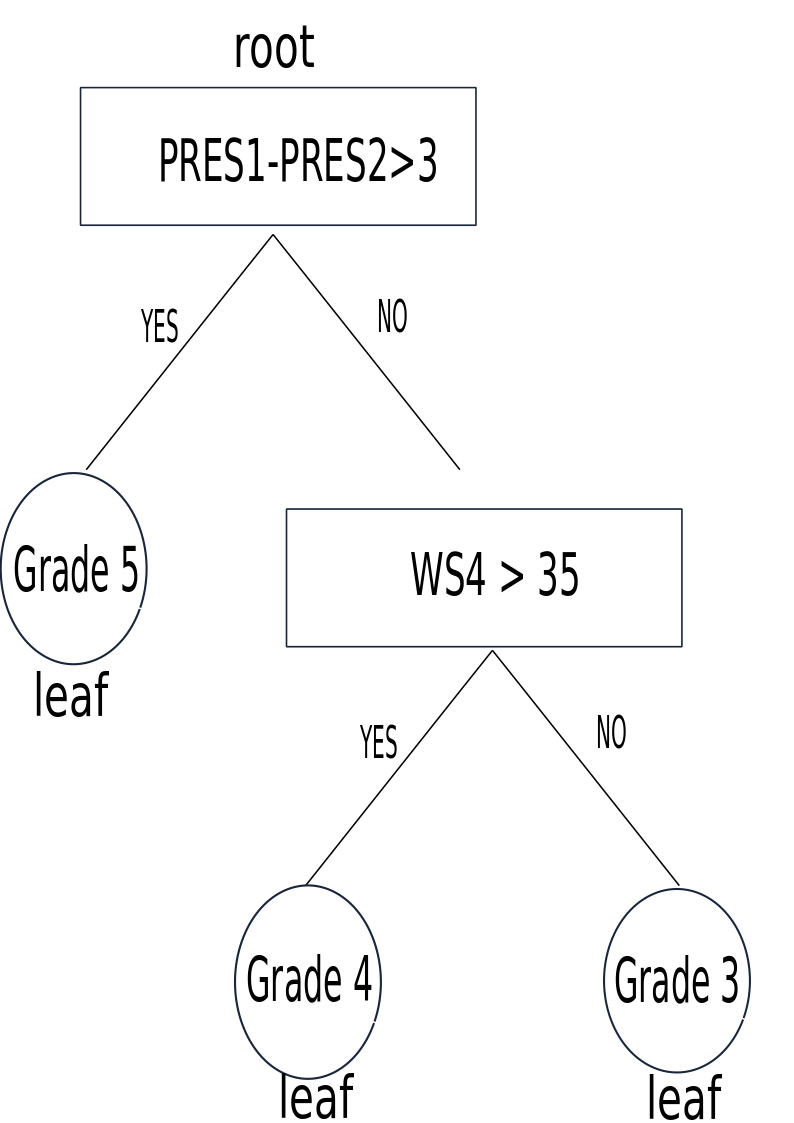
\includegraphics[width=3in,height=1.75in]{SimpleDecTree.png}
	\caption{Simple example of a decision tree used to classify typhoon grade.}
	\label{SimpleDecTree}
\end{figure}

A Random forest algorithm uses $N$ decision trees and selects the majority category. By increasing the number of leaves in the Decisions trees, a classification algorithm becomes a type of regression model.

\subsection{Support Vector Machines (SVM)}
The idea of support vector machines (SVM), a type of ML algorithm mainly applied to classification problems,  is to use hyperplanes to separate predictors into categories as shown in Figure \ref{SimpleSVM}. An optimal hyperplane maximizes the distance between the separated categories. In some cases, a transformation of the data is needed before SVM can be applied. 

\begin{figure}[!htpb]
	\centering
	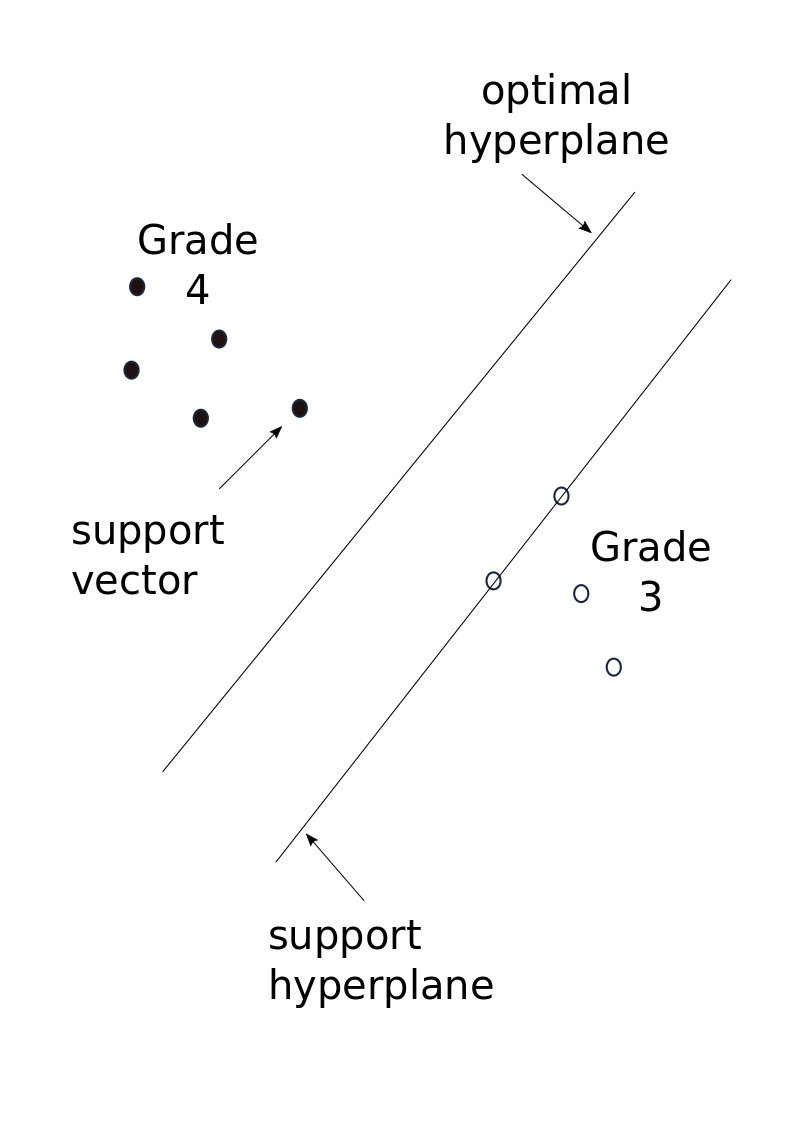
\includegraphics[width=3in,height=1.75in]{SimpleSVM.png}
	\caption{Simple illustration of SVM classification.}
	\label{SimpleSVM}
\end{figure}

\subsection{K Nearest Neighbors (KNN)}
The K Nearest Neighbor algorithm (KNN) assigns a category based on the k closest predictors. In the case of classification, the category with the highest frequency among the K neighbors is selected. In the case of regression, an average of the k closest predictors may be used. Different choices of K may be investigated to give the best separation between categories.


\begin{figure}[!htpb]
	\centering
	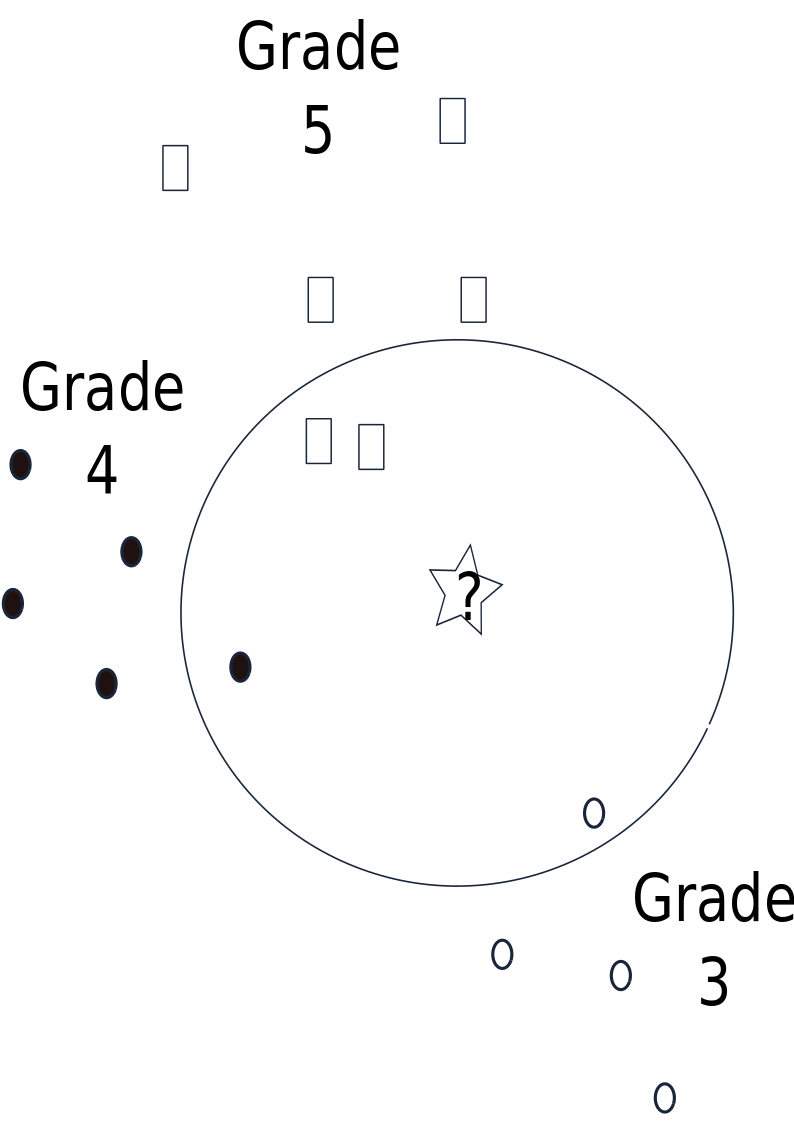
\includegraphics[width=2.25in,height=3in]{SimpleKNN.png}
	\caption{Simple illustration of KNN classification. In this case K=4.}
	\label{SimpleSVM}
\end{figure}

\subsection{Ensemble}
The ensemble method \cite{Diet} takes a set of individual algorithms and combines them in some way, for example by a majority classification or a weighted average of regression values.  An important research area in supervised ML is development of methods to construct good ensembles.

\newpage

\section{Exercises}  

\begin{enumerate}
	\item What is the overall percentage of correct typhoon grade prediction based on the information in an ensemble model ML confusion matrix shown in Figure \ref{EnsembleClass}? How well does the model predict grade 5 typhoons (give percentages of correct, false positives and false negatives).)
\begin{figure}[!htpb]
	\centering
	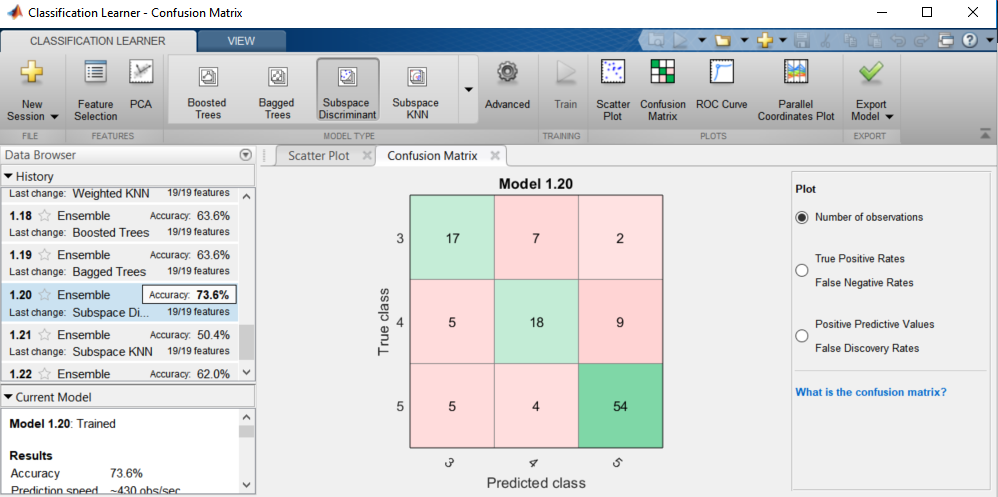
\includegraphics[width=3in,height=1.75in]{Ensemblefig1.png}
	\caption{Confusion matrix for a MATLAB subspace discriminant ensemble classification algorithm.}
	\label{EnsembleClass}
\end{figure}

\item An \emph{accurate} classifier is one that has an
error rate of better than random guessing on new {\bf x} values. Two classifiers are \emph{diverse} if they make different errors on new data points. Prove that a necessary and sufficient condition for an ensemble of classifiers to be more
accurate than any of its individual members is if the classifiers are accurate and
diverse. (See \cite{Hansen}.
 

\end{enumerate}
\newpage
\section{Computer Project}
{\flushleft Project website: 
https://www.overleaf.com/project/5c057323a87843644f4893a6}


MATLAB has a Statistics and Machine Learning Toolbox which has apps to build both categorical and regression model.  The main steps in creating these ML models are:

\begin{itemize}
	\item Train MATLAB's suite of ML models using a specified dataset.
	\item Choose one of the models with high accuracy, and export a MATLAB function based on your selected trained model.
	\item Apply the exported model to a validation dataset.
	 If satisfied, continue to the next step. If not, repeat the previous steps.
	 \item Test the model on a new data set and record the error. 
	\end{itemize} 

\begin{enumerate}
 \item Using the CategoryTrainingData.xlsx and CategoryData15.xlsx for training and validation data sets respectively, use MATLAB to develop a ensemble categorical ML model for typhoon grade. Include the confusion matrices in your report. 
 \item Using the RegressionTrainingData.xlsx and RegressionData15.xlsx and a KNN regression model or training and validation data sets respectively, use MATLAB to develop  a ML regression model for the time where the maximum wind speed is first attained on the best track. Include a residual error analysis in your report.
\end{enumerate}

\emph{Project Team:} Michaela Flitsch, Mark Nussbaum, Zach Oslund, Matthew Rueger.

\newpage
 \begin{thebibliography}{9}

 \bibitem{Bon}  {Bonnardot, G.}, 8 Machine Learning Algorithms Explained in Human Language. Available at https://www.datakeen.co/en/8-machine-learning-algorithms-explained-in-human-language/
 
 \bibitem{Diet} {Dietterich, T.} Ensemble Methods in Machine Learning.  Available at http://web.engr.oregonstate.edu/$\sim$tgd/publications/mcs-ensembles.pdf
 
 \bibitem{Hansen} {Hansen, L. and Salamon, P.} Neural network ensembles. 1990. IEEE Trans. \emph{Pattern Analysis and Machine Intell}, 12, 993-1001.
 
\bibitem{JMA} {Japan Meteorological Agency},  Best track archives. Available at  http://www.jma.go.jp/ jma/jma-eng/ jma-center/ rsmc-hp-pub-eg/trackarchives.html.

\end{thebibliography}
\end{document}
%
%\item Japan Meteorological Agency, 2014: {\em Annual Report of the RSMC Tokyo-Typhoon Center 2013}. http://www.jma.go.jp/jma/ jma- eng/jma-center/rsmc-hp-pub-eg/AnnualReport/2013/Text/Text2013.pdf
%
%
%\item Jin, L., C. Yao and X. Huang, 2008: A Nonlinear Artificial Intelligence Ensemble Prediction Model for Typhoon Intensity. \emph{Mon. Weather Rev.}, {\bf 136}, 4541-4554.
%
%\item Knaff, J.A., C.R. Sampson, and M. DeMaria, 2005: An operational statistical intensity prediction scheme for the western north Pacific. \emph{Weather Forecast.}, {\bf 20}, 688-699.
%
%
%    \item Komaromi, W.A., S.J. Majumdar and E.D. Rappin, 2011: Diagnosing initial condition sensitivity of typhoon Sinlaku (2008) and hurricane Ike (2008), {\bf 139}, 3224-3241.
%
%\item  Korean Meteorological Administration, 2013: {\em Annual Report}. \\ http://web.kma.go.kr/download\_01/Annual\_Report\_2013.pdf
%
%\item Krishnamurti, T.N., J. Xue, H.S. Bedi, K. Ingles, and D. Oosterhof, 1991: Physical initialization for numerical weather prediction over the tropics. \emph{Tellus}, {\bf 43}, 53-81.
%
%\item Krishnamurti, T.N., C.M. Kishtawal, T.E. LaRow, D.R. Bachiochi, Z. Zhang, C.E. Williford, S. Gadgil, and S. Surendran, 1999: Improved weather and seasonal climate forecast from multi-model superensemble. \emph{Science}, {\bf 285}, 1548-1550.
%
%\item Leith, C.E., 1974: Theoretical skill of Monte-Carlo forecasts. \emph{Mon. Wea. Rev.,} {\bf 102}, 409-418.
%
%\item Leslie, L.M., R. Abbey and G.J. Holland, 1998. Tropical cyclone track predictability. \emph{Meteorol. Atmos. Phys.}, {bf 65}, 223-231.
%
%\item Lorenz, E.N., 1963: Deterministic nonperiodic flow. \emph{J. Atmos. Sci.}, {\bf 20}, 130-142.
%\item Lorentz, E.N., 1965: A study of the predictability of a 28-variable atmospheric model. \emph{Tells}, {\bf 17}, 321-333.
%
%\item Meng, Z. and F. Zhang, 2007: Tests of an ensemble Kalman filter for mesoscale and regional-scale data assimilation. Part II: Imperfect model experiments. \emph{Mon. Weather Rev.,} {\bf 135}, 1403-1423.
%
%\item Neumann, C. J., 1972: An alternate to the HURRAN tropical cyclone forecast system. \emph{NOAA Tech. Memo.} NWS SR-62, 22 pp.
%
%\item  Rozanova, O. S., J.-L. Yu, and C.-K. Hu, 2010: Typhoon eye trajectory based on a mathematical model: comparing
%with observational data. \emph{Nonlinear Analysis: Real World Applications.} {\bf 11}, 1847�1861.
%
%\item $\ddot{\textup{U}}$ster, H. and R.F. Love, 2001: Application of a weighted sum of order $p$ to distance estimation. \emph{IIE Trans.}, {\bf 33}, 675-684.
%
%\item Weber, H., 2005: Probabilistic prediction of tropical cyclones. part 1: position. \emph{Mon. Weather Rev.}, {\bf 133}, 1840-1852.
%
%\item Williford, C.E., T.N. Krishnamurti, R.C. Torres, and S. Cocke, 2003: Real-time multimodel superensemble forecasts of Atlantic tropical systems of 1999. \emph{Mon. Weather Rev.}, {\bf 131}, 1878-1894.
%
%\item Wu, C.-C., and K. Emmanuel, 1993: Interaction of baroclinic vortex with background shear: application to hurricane movement. \emph{J. Atmos. Sci.}, {\bf 50}, 62-76.
%
%    \item Yamaguchi, M., T. Nakazawa, and K. Aonashi, 2012:  Tropical Cyclone track forecasts using JMA model with ECMWF and JMA initial conditions. \emph{Geophys. Rev. Lett.,} {\bf 39}, L09801, doi:10.1029/2012GL051473.
%
%\item Yanase, W., H. Taniguchi, M. Satoh, 2010: The genesis of tropical cyclone Nargis (2008): environmental modulation and numerical probability. \emph{J. Meteor. Soc. of Japan}, {\bf 88}, 407-519.
%
%        \item Yang, S.-C., E. Kalnay and T. Miyoshi, 2012: Accelerating the EnKF spinup for typhoon assimilation and prediction. \emph{Weather Forecast.}, {\bf 27}, 878-897.
%
%\end{list}

%Official annual tropical storm and typhoon best track data (lat, lon, windspeed, pressure in 6 hour time increments) is published by the Japan Meteorological Agency (JMA). To develop a best track prediction model, you are allowed to use as your training data the JMA best track data for the thirteen typhoons Soulik, Utor, Manyi, Usagi, Wutip, Fitow, Dana, Nari, Wipha, Francisco, Lekima, Krosa, and Haiyan in 2013  available at
%  \\ {\scriptsize http://www.jma.go.jp/jma/jma-eng/jma-center/rsmc-hp-pub-eg/besttrack.html}.
%{\flushleft Design} a model such that given just the 2013 training data and the initial best track point of the eleven typhoons in 2014 shown in the table below, you can predict the best track position of each 2014 typhoon at the 120 hour mark with an average error of less than 500 km.
%
%\begin{table}[!htpb]
%\scriptsize
%\centering
%\begin{tabular}{|c|l||c|c|c|c|}\hline
% Typhoon& International&\multicolumn{4}{|c|}{Initial best track}\\
%        & I.D. &lat & lon & pressure  & wind speed\\\hline
% Faxai&1403&8.7&147.8&1004&0\\\hline
% Neoguri& 1408&8.4&146.8&1006&0\\\hline
% Rammasun &1409&8.0&154.3  &1006&0\\\hline
% Matmo& 1410&10.0&136.8&1006&0\\\hline
% Halong  & 1411&11.3 &151.8& 1006&0\\\hline
% Genevieve  & 1413&13.6 &181.2& 950&0\\\hline
% Kalmaegi&1415&13.5 &134.0&1004&0\\\hline
% Phanfone   & 1418 &11.0& 157.1&1004&0\\\hline
% Vongfong &  1419&7.3 &162.1&1006&0\\\hline
% Nuri & 1420&12.6 & 140.9&1004&0\\\hline
% Hagupit& 1422&2.6&156.0&1006&0\\\hline\hline
%  \end{tabular}
%  \caption{ Initial best track points of typhoons in 2014.}
%  \end{table}
%
%\vspace{.3in}
%
%
\end{document}